\documentclass[10pt,b5jsbook,dvips,dvipdfmx,openany]{jsbook}

\usepackage[explicit]{titlesec} %章立てのレイアウト変更
\usepackage{picture} %色付きの箱を作ったり
\usepackage[usenames]{color} %好きな色を作れます
\usepackage{amsmath}%数式を使うならまずこれ!
\usepackage{amssymb}%特殊な記号を使いたいならとりあえずこれ!
\usepackage{mathrsfs}%カッコいい花文字を使うときはこれ!
\usepackage{bm} %ベクトルとか数式の太字
\usepackage{braket} %ブラケットを作るには必要
\usepackage{tikz} %texで図を書く場合などに用いる.
\usepackage{amsfonts}
\usepackage{enumitem}
\usepackage{dsfont}
\usetikzlibrary{calc}
\usetikzlibrary{decorations.markings,decorations.pathmorphing}
\usepackage{url} %外部リンク生成
\usepackage{multicol} \setlength{\columnseprule}{0.4pt}
 \usepackage{multirow}
 %\usepackage{MnSymbol}

%\usepackage{mathabx}%小文字の筆記体を使うときはこれ!(予め, パッケージをダウンロードすること.  )

%--------------------------------------------------
%定義, 定理等(どれかを使うと便利) %パンフでは多分そんなに使わない
\usepackage{amsthm}
\theoremstyle{definition}
  \newtheorem{theorem}{定理}[section]
  \newtheorem{definition}[theorem]{定義}
  \newtheorem{lemma}[]{補題}
  \newtheorem{corollary}[theorem]{系}
  \newtheorem{proposition}[theorem]{命題}
  \newtheorem{example}[theorem]{例}
  \newtheorem{formula}[theorem]{公式}

%\usepackage[usenames,divpsnames]{xcolor}

%------------------------------------------------
% colors %好きに足すといいと思います
\definecolor{oldrose}{RGB}{219, 86, 115}
\definecolor{spinelred}{RGB}{235,121,136}
\definecolor{sakura}{RGB}{242, 216, 223}
\definecolor{teal}{RGB}{0,128,128}
\definecolor{mauve}{RGB}{133, 88, 150}
\definecolor{powderblue}{RGB}{176,224,230}
\definecolor{darkslateblue}{RGB}{72,61,139}
\definecolor{darkslategray}{RGB}{47,79,79}
\definecolor{lightcyan}{RGB}{224,255,255}
\definecolor{red}{RGB}{250, 0, 0}
\definecolor{toki}{RGB}{236, 165, 178}

%------------------------------------------
%見た目の変更. chapterとかsectionとか

%基本形----------------------------------
%\titleformat{変更する階層(sectionとか)}
%   [形状など(デフォルトはhang)]
%    {書式(フォントなど) }
%    {<ラベル書式>}
%    {<ラベルと見出し文字列の間の空き>}
%    {<見出し文字列直前に入るコード>}
%    [<見出し直後に入るコード>]

% chapter------------------------
\titleformat{\chapter} %変更する階層
[hang] %形状など
{\vspace{-25truemm} \HUGE} %書式(フォントなど)
{} %ラベル書式
{0pt} %ラベルと見出し文字の間の空き
{\titleline[r]{#1} \titlerule} %見出し文字直前
[\vspace{-10mm}]%見出し直後

% section----------------------------------
\titleformat{\section}[block]
{\Huge}{}{0pt}
{\hspace{-2mm}
  \colorbox{mauve}{\begin{picture}(0,16)\end{picture}}%\thesection
  \hspace{0pt}  \normalfont #1}
[
\begin{picture}(100,0)
  \put(2,30){\color{mauve}\line(1,0){300}}
\end{picture}
\\
\vspace{-50pt}
] 

% subsection--------------------------------
\titleformat{\subsection}[block]
{ \normalfont \Large}{}{0pt}
{\hspace{-1mm}
  \colorbox{toki}{\begin{picture}(0,10)\end{picture}}
  \hspace{0pt}
 \bfseries %\thesubsection
  \hspace{-4pt} #1
}
[
\begin{picture}(100,0)
  \put(2,18){\color{toki}\line(1,0){200}}
\end{picture}
\\
\vspace{-40pt}
]



% 余白の大きさを決める. 
\usepackage[top=30truemm, bottom=20truemm, left=20truemm, right=20truemm]{geometry}

%-------------------------------------------------
%画像関連
\usepackage{graphicx}
\usepackage{wrapfig}%これを使えば, 図の周りに文字を回り込ませることができる.
%横向きを使うときは下も使う
%\usepackage{lscape}s

%--------------------------------------------------
%柄つきの枠(アクセントなどにどうぞ!)
\usepackage{fancybox}
\usepackage{tcolorbox}
\usepackage{ascmac}

%--------------------------------------------------
%しおり, リンク等
%(pdfファイルにしおりや内部リンクを自動生成させます.  コンパイルできない時などは消してください.  )
\usepackage[dvipdfmx, colorlinks=false, bookmarksnumbered=true, linkcolor=blue]{hyperref}
  %\AtBeginDvi{\special{pdf:tounicode 90ms-RKSJ-UCS2}}
\AtBeginDvi{\special{pdf:tounicode EUC-UCS2}}

%\title{入寮募集要項}

\begin{document}
  %\maketitle
   
\setcounter{page}{1}
  \pagenumbering{arabic}
  \setcounter{tocdepth}{1}
  \tableofcontents

    \thispagestyle{empty}

  \newpage
 

\chapter{入寮にあたって}
	\section{熊野寮概要} \label{sec:abst}

		\subsection{基本データ} \label{subsec:data}
		\begin{description} 
		\item[寮費] \hspace{10mm}
			\begin{description}
			\item[維持費] 月4,100円(水光熱費込み)
			\item[入寮予備金] 3,000円
			\end{description}
		\item[寮食] \hspace{10mm} 
			\begin{description}
			\item[内容] 基本的に朝昼夕の三食
			\item[期間] 授業期間の平日(土日祝は休み)
			\item[食券代] 朝180円, 昼290円, 夕420円(5食分以上のまとめ買いのカードなら朝10円, 昼夜は30円引き)
			\end{description}
		\item[連絡先] \hspace{10mm} 
			\begin{description}
			\item[住所]606-8393 京都府京都市左京区丸太町通川端東入東竹屋町50 京都大学熊野寮
			\item[電話番号] 075-751-4050 または 075-751-4051
			\end{description}
		\end{description}

    %\begin{wrapfigure}[0]{r}[0pt]{0.5\textwidth}
  	%	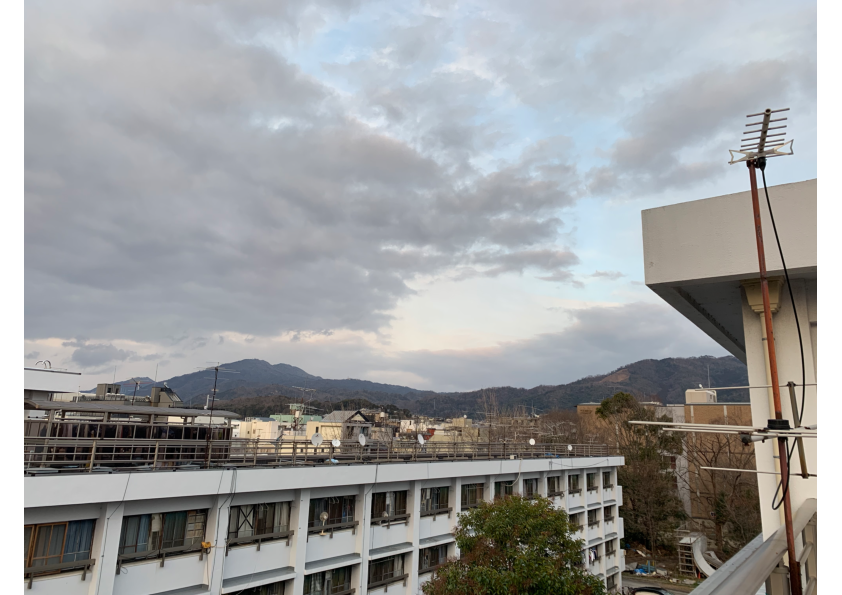
\includegraphics[scale=0.3]{terrace.pdf}
  			%\caption{}
  	%		\vspace*{-\intextsep}
  	%		\label{fig:屋上}
  	%		\end{wrapfigure}

		\subsection{建物概略}
		\begin{description}
		\item 4階建て鉄筋コンクリート3棟(A棟, B棟, C棟, 食堂)
		\item 築約50年, 各階11部屋(例外あり), 総部屋数127
		\item[定員] 422名
		\item[居室] A棟16畳,  B棟18畳(定員4名), C棟(定員2名)\footnote{C棟は3部屋を6人で用いるなどしています}
		\item[備品] 事務机, 椅子, 本棚, 二段ベッド, クローゼット
		\end{description}



%ここに建物の写真か何か入れる % やっぱやめる

 \newpage

		\subsection{共同設備}
		\begin{description}
		\item[居室内]冷蔵庫やテレビ, 電気ケトル, 炊飯器などは上回生が持っていたり, 部屋で受け継がれていたりする場合がある. 防災上, 石油ストーブは禁止. 寮内は屋上含め全面禁煙. 喫煙所が玄関脇にある.
		\item[談話室]各階に設けられた十数畳の部屋. 各階の集会場兼遊戯室となる. 使用状況は階によって様々だが, たいてい漫画$ \cdot $ ゲームなどが置いてある.
		\item[炊事場]各階にある. ガスコンロ$ \cdot $ ガス湯沸かし器$ \cdot $ 流し$ \cdot $ 鏡などがある.
		\item[洗濯機]各階にある. 各棟屋上には物干し場と乾燥機がある.
		\item[トイレ]各階にある. 男女別の水洗トイレ. 和$ \cdot $ 洋式どちらもある. B棟一階には多目的トイレがある.
		\item[食堂]栄養士さんが考えたバランスのとれた食事を, 日替わりで楽しめる. 食堂内には自動販売機, 製氷機, 電子レンジがある. 卓球台も置いてある. 食堂はコンパなど多くの催し物に使われる.
		\item[事務室]維持費の支払い, 来客の対応などをする. 新聞各紙(京都$ \cdot $ 読売$ \cdot $ 朝日$ \cdot $ 毎日$ \cdot $ 日経) を閲覧できる. ここでは常時寮生が事務室当番として電話の取次ぎや, 郵便物の管理を行っている.
		\item[シャワー]A棟一階には男女別のシャワー個室があり, 男子6基, 女子2基ある. 料金は3分10円のプリペイドカード式. ドライヤーもある.
		\item[ロビー]食堂に準ずる交流の場. コンパなどに利用される.
		%\item[軟鉄庵]青い光の灯る隠れ家的共有スペース. BARなどに利用される. 本も置いてある.
		\item[音楽室]B棟地下にある, スタジオ兼ライブハウス. %格安ライブハウス. 寮外生も利用できる.
		\item[硬鉄庵]B棟地下にある, 分厚い扉に守られた部屋. 警察権力からの防衛に特化している.
		\item[民青池]たまに飛び込む者がいる. 寮祭企画$ \cdot $ みかん祭りの開催場所になったりもする. 元々は消火用.
		\item[娯楽]食堂の卓球台, 敷地内のバスケットゴール$ \cdot $ フットサルコートなどに加え, 部屋で受け継がれているものもある.
		\end{description}

    \begin{figure}[h]
    		\begin{flushleft}
     	 	\includegraphics[scale=0.3]{muc.pdf}
    		\end{flushleft}
    		\end{figure}


\newpage
	\section{募集要項} \label{sec:gl}
		\subsection{募集対象}
		京都大学の学生, 大学院生, 研究生, その他本学に学籍のある者(科目等履修生, 聴講生など)を対象とする. 性別, 国籍は問わない.

		\subsection{募集人数}
		現在の空き人数(100名程度)を募集する.

		\subsection{選考}
		入寮希望者が募集人数を超えた場合には選考を行う.
		\begin{description}
		\item[入寮基準]
		寮自治活動を理解し, 積極的に参加すること.
		\item[選考方法]
		部屋割りの都合上, 選考は男女に分けて行われる.
			\begin{description}
			\item[一般選考]全員に対して抽選を行って選考する.
			\item[特別選考] 一般選考に優先して行われる.
	\end{description}
	\begin{itembox}[l]{\bf 特別選考の内容}

		\begin{description}
		\item[経済選考] 経済的に困窮している者は, 経済選考に出願できる. 出願希望者は, 出願参考書類の所定の欄に記入し, 既定の書類(後述)を添えて提出すること. 困窮状況が明らかな場合は優先的に入寮を認める.
		\item[留学生選考] 留学生は経済選考で必要な証明書を提出するのが困難であること, また留学生が置かれている社会的状況を考慮し, 留学生枠を設定する. 経済的に困窮している留学生の入寮希望者は, 留学生枠への応募が可能である. その際, 留学生選考用書類も併せて提出する必要がある. 応募者の総数が留学生枠を超えた場合は, 留学生枠内で抽選を行う.
		\end{description}

なお, 上記の経済選考, 留学生選考に応募した者は, 経済選考$ \cdot $ 留学生選考に漏れた時点で自動的に一般選考にまわる.

	\end{itembox}

	\end{description}

			\subsubsection{前$ \cdot $ 後期枠の区別と定員配分}
			前期$ \cdot $ 後期の二つの枠を設け選考する. 前期枠は2/25$ \sim $ 3/16の面接日に出願してきた者, 後期枠は3/23$ \sim $ 3/24の面接日に出願してきた者を対象とする.

			後期枠は, 合格発表が遅い後期特色入試での入学者が入寮を希望する場合も考慮して設けられているものである. 後期特色入試での入学者以外が後期枠に出願することも可能だが, 選考においては後期特色入試での入学者を優先する. 前期枠に比べて後期枠の定員は少なくなっているが, 前期枠に空きが生じた場合はその分を後期の定員に追加する.

\newpage % これはレイアウトの都合なのでいらなさそうなら消す

		\subsection{出願書類}

 		下記の書類を面接時に提出すること. なお, 一度提出された書類はいかなる理由があろうと返却しない. \footnote{原則面接日に提出すること. やむを得ず当日用意できない事情がある場合は, 面接受付時にその旨を申し出たうえ, 入寮手続きまでに必ず提出すること. }

 		\begin{itembox}[l]{\bf 全員必要なもの}
		\newcounter{mymemory}
		\begin{enumerate}
		\item \textbf{学籍を確認できるもの(学生証など) の写し.} \footnote{受験生は入試当日は受験票を持参のこと. 入寮手続き時に合格証明書の写しなどを提出}
		\item 入寮願(署名と捺印のうえ, 顔写真を貼ること )※留学生は捺印不要
		\setcounter{mymemory}{\value{enumi}}
		\item 同一世帯の住民票の写し(発行日から3ヶ月以内のもの) ※留学生は不要
		\item 出願参考書類(顔写真を貼ること)
		\end{enumerate}
		\end{itembox}

		また, 特別選考に応募するものは上記の書類に加えて, 選考区分に応じて以下の書類を提出すること.


		\begin{itembox}[l]{\bf 特別選考書類}

		\begin{description}
		\item[経済選考出願に必要な書類]

		提出期限は以下の通り厳守のこと.
			\begin{description}
			\item[前期]3月16日17時
			\item[後期]3月24日17時
			\end{description}

			\begin{enumerate}
			\setcounter{enumi}{\value{mymemory}}
			\item 同一世帯の住民票の写しも必ず提出のこと
			\item 出願参考書類\footnote{所定の欄に経済状況(家族の人数, 収入の有無, 就学の状況など)についての説明をできるだけ詳細に記入すること. 十分な情報が記されていない場合, 経済選考に出願できない場合がある. }
			\item  家族全員の所得(または家庭の経済状況)を示すことのできる公的機関の発行する証明書(コピー可) \footnote{例: 源泉徴収票, 確定申告書, 失業保険の給付証明書, 住民税の免除証明書など. }
			\item 特別な事情がある場合には, そのことを詳しく書いた書類やそれを証明できる公的な書類
			\setcounter{mymemory}{\value{enumi}}
			\end{enumerate}

		\item[留学生選考出願に必要な書類]

			\begin{enumerate}
			\setcounter{enumi}{\value{mymemory}}
			\item 留学生選考書類
			\end{enumerate}
		\end{description}

		\end{itembox}

		\subsection{面接}
		入寮を希望する者は, 必ず入寮面接を受けなければならない. この面接は入寮希望者が予め寮自治について理解するために行われる. これによる選考は, あまりに寮自治への理解がないと判断される場合を除いて行わない.

		\begin{description}
		\item[面接日時] 面接は前期と後期の2回に分けて行われる. %複数の日程があるが, 選考については, 前期枠は3月16日, 後期枠は3月24日にまとめて行われる.

\begin{table}[htb]
  \begin{tabular}{|l|c|c|c||l|c|c|c|} \hline
    		& 日程 & 受付時間  & 当落連絡 &	& 日程 & 受付時間 & 当落連絡 \\ \hline \hline
    \multirow{6}{*}{前期}
      		& 2月25日(月)& \multirow{2}{*}{15:00 $ \sim $ 17:00 }& \multirow{6}{*}{3月17日(日)} &\multirow{6}{*}{後期} & &  \multirow{6}{*}{10:00 $ \sim $ 17:00} & \multirow{6}{*}{3月25日(月)} \\
    		& 2月26日(火)&  & & & & &\\ \cline{2-3}
      		& 3月10日(日)&  \multirow{4}{*}{10:00 $ \sim $ 17:00}& & & 3月23日(土) & &\\
    	  	& 3月11日(月)& & & & 3月24日(日)& &\\
      		& 3月12日(火)& & & & & &\\
     		& 3月16日(土)& & & & & &\\ \hline
  \end{tabular}
\end{table}


%表の記述は改善の余地あり
		\item[所要時間] $1 \sim 2 $ 時間
		\item[寮内見学] 面接後に可能である. 面接の場に入寮希望者本人以外は同席できないが, 見学は付添人の同伴も可能である. なお, 付添人には面接中の待合スペースを用意している.
		\end{description}

		\subsection{選考後の流れ}
		\begin{enumerate}
		\item 当落発表

		面接最終日の夜に選考を行う. 翌日中, 18時までに, 当落に拘わらず全ての出願者に選考結果を電話で通知する.
		\item 繰り上げ当選

 		落選者は, キャンセル待ちに登録することができる. 選考結果の連絡を受けた際に申し込むこと.

 		選考当選者のキャンセルが発生するたびに, キャンセル待ちに登録した者の中から, 繰り上げで追加の当選者が確定していく. 追加で当選した者には, 当選した時点で電話で連絡する.
		\end{enumerate}

		\subsection{入寮手続き}
		期日までに行われなければ入寮資格を失う. やむを得ず面接日に不足書類があった者は手続きまでに必ず書類を持参すること.
			\subsubsection{受付日}  3月に以下の日程で受け付けている. %場所はかかんでええのかね
			\begin{table}[h]
\begin{tabular}{|l|l|c|l|c|}
\hline
\multicolumn{2}{|c|}{受付日} & 曜日  & \multicolumn{2}{|c|}{受付時間}                  \\ \hline \hline
18日         & 25日        & 月 & 9:45 $ \sim $ 12:45 & $ \times $           \\ \hline
19日         & 26日        & 火 & 9:45 $ \sim $ 12:45 & 14:00 $ \sim $ 15:30 \\ \hline
20日         & 27日        & 水 & 9:45 $ \sim $ 12:45 & $ \times $           \\ \hline
21日         & 28日        & 木 & 9:45 $ \sim $ 12:45 & 14:00 $ \sim $ 15:30 \\ \hline
22日         & 29日        & 金 & 9:45 $ \sim $ 12:45 & 14:00 $ \sim $ 15:30 \\ \hline
\end{tabular}
\end{table}
\subsubsection{入寮オリエンテーション}
			3月30日(土)14時からの入寮オリエンテーションに参加すること. また, これに不参加の者は強制退寮となる場合があるので, 必ず参加のこと.

			所要時間: 3時間程度

%以下英語版. 本誌に掲載する場合はコメントアウトを解除する
%\section{Admission Guidelines for International Students}

%\subsection{Who is eligible:}
%A student who studies at Kyoto University (who has been accepted to attend a certain course of the university or the graduate school). Japanese language proficiency to hold daily conversations is highly recommended.

%\subsection{Application:}
%Those who wish to enter Kumanoryo will be asked to understand and actively participate in our self-government association. If the number of people who want to join Kumanoryo exceeds the number of places available, we draw lots to decide.

%\subsection{Application documents:}
%Please submit the following documents at the interview. Furthermore, we will not return any submitted documents for any reason. If you are unable to provide them at the interview, please send them by the designated date upon discussing with the interviewer.

%\begin{enumerate}

%\item Application form (enclosed with this pamphlet. Can also be downloaded from the website)
%Please sign and paste a photograph of your face.

%\item A photocopy of a document that identifies your registration to university, such as a student ID

%\item Documents for students from outside of Japan (enclosed with this pamphlet. Can also be downloaded from the website)

%\end{enumerate}

%\subsection{Interview:}
%You will have to go for an entry interview. This interview is conducted so that you will have a thorough understanding of the facility. You will also be informed about the rules here, and if you are deemed not to be willing to perform your duty, you might not be able to enter the dormitory, so please take note of this.

%\begin{table}[htb]
  %\begin{tabular}{|l|c|c|c||l|c|c|c|} \hline
    		%& Dates & Hours  &  && Dates & Hours  &   \\ \hline \hline
  %  \multirow{6}{*}{}
      	%	& Feb. 25th & \multirow{2}{*}{15:00 $ \sim $ 17:00 }& \multirow{6}{*}{Mar. 17th} &\multirow{6}{*}{} & &  \multirow{6}{*}{10:00 $ \sim $ 17:00} & \multirow{6}{*}{Mar. 25th} \\
    	%	& Feb. 25th &  & & & & &\\ \cline{2-3}
      	%	& Mar. 10th &  \multirow{4}{*}{10:00 $ \sim $ 17:00}& & & Mar. 23th & &\\
    	 % 	& Mar. 11th & & & & Mar. 24th& &\\
      	%	& Mar. 12th & & & & & &\\
     	%	& Mar. 16th & & & & & &\\ \hline
 % \end{tabular}
%\end{table}
     %Time needed: 1-2 hours (you can have a tour of the dormitory after the interview)

%\subsection{Results}
%The screening result would be emailed to you between 10 a.m. and 6 p.m. on March 17th. If you would like to decline entering Kumanoryo, please contact us as soon as possible. If you were not selected, you can also register to wait for cancellations. If there is a cancellation made by a successful applicant, we will contact those who have been additionally selected by email.

%\subsection{Check-in:}
%Please come to Kumanoryo to complete the entering process on one of the following dates, and participate in the orientation to be held on hogehoge. If the dates do not fit your schedule, please contact us.


\chapter{寮での生活} % 仮称.

	\section{寮食堂と寮生}	\label{sec:cafeteria}
 	熊野寮には, 全国の学生寮でも数少ない寮食堂があります. 基本的に大学の授業がある平日, 朝昼夜の三食が用意され, 朝は7時半$\sim$10時, 昼は12時 $ \sim $ 13時, 夜は17時$ \sim $ 17時30分が喫食時間としています. これを見て, 「え, そんなに食べる時間短いの? 」と思った方もいるでしょう. ご安心を, そういったご飯の時間内には食べに来られない人のために昼と夜は「残置」というシステムを作ってあり, 昼は15時まで, 夜は22時までに食べにくるという条件の下で寮食を取り置くことができます! さらに, 寮食には利点がいっぱいあります!

		\subsection{寮食は栄養満点! }
 		まず, 寮食堂には栄養士の方がいらっしゃり, 毎日の栄養計算から献立を作って下さっています. しかもボリュームも満点! しっかり三食食べれば二十歳の成人男性が一日に必要な栄養素を摂取できるのです. 朝はパンと乳製品, 昼は野菜たっぷりのご飯, 夜は主菜を中心とした汁物, 副菜二品セット. 寮食三食で一日分のビタミン, ミネラルも摂取できるのです. 今の若い時分にしっかり栄養を摂っておかないと将来生活習慣病の予備軍になってしまいますが, 寮食なら安心ですね.

		\subsection{寮食は安全安心! }
寮食は安全面にも気を配っています. 衛生面はもちろんのこと, 使う材料にも気を付けており, 肉はほとんど国産, 野菜は京野菜をふんだんに使用し, 卵は餌から管理されているものを使い, 添加物も極力省いています. 栄養面でも安全性の面でも身体に良い寮食, これは食べるしかありませんね!

		\subsection{寮食は安い!}

		栄養満点ボリューム満点, おまけに安全安心そんな寮食. でもお高いんでしょう? いえいえ, そんなことはありません! \emph{朝は170円, 昼は260円, 夜は390円と破格! }しかしながらその裏には厨房の栄養士さんや調理員さんの多大なる努力があります. 食材を大量購入し, その材料が無駄にならないような調理法, 献立を考えた上で栄養も毎日しっかり保つ. さらには夏の冷麺や素麺, 冬の鍋物やシチュー, おまけに節分(2月3日) やバレンタイン(2月14日) などの季節を感じさせるメニューも登場します.

		\subsection{寮食堂は交流の場}
		食堂と言えばご飯を食べるところ. もちろんそれが食堂の一番の意味ですが, 熊野寮食堂は様々な寮生と知り合い交流する場でもあります. 熊野寮の食堂は24時間365日開放されています. その管理$ \cdot $ 運営は寮生と厨房員さんの二人三脚で行われます. なので自分たちの好きな時に自分たちの好きなことができる. これこそまさに自治であり, 寮食堂とは自治を象徴する場所なのです! 他愛もない話から昨今の政治の動きなどの難しい話まで, 色んな話をしながら寮食を食べるのもあり. 時々企画されるコンパやイベント事で朝まで交流するのもあり. 炊事当番(食器洗い当番とも言う) では寮生や厨房の方と一緒に働く. 自分たちの意志で自由にできる場所です. そしてその意思決定には外部からの干渉は受けません! 友達ができそうになくボッチになりがちな人でも, 寮食を食べたりコンパやイベントに参加したりすれば, 楽しい出会いが待っていることでしょう.

		ここだけでは熊野寮食堂の素晴らしさは語りつくせません. 入寮した暁には, 寮食共々是非食堂を利用して有意義な大学生活を送って下さい.

		\subsection{寮食メニュー例}

\begin{table}[htb]
\begin{tabular}{|c|c|c|c|c|c|} \hline
&月&火&水&木&金 \\ \hline \hline
朝食& \multicolumn{5}{|c|}{パン, 乳酸飲料, チーズor卵} \\  \hline \hline
\multirow{6}{*}{昼食} & チキンカツ丼 &カレーピラフ & ハヤシライス & 柳川風丼 & 桜寿司 \\
&&サラダ	&ヨーグルトサラダ&ごま和え&ごま和え \\
&&コーンスープ&&&かき卵汁 \\  \cline{2-6}
&&長崎ちゃんぽん&&&にしんそば \\
&&&&&ごま和え \\  \cline{2-6}
&\multicolumn{5}{|c|}{火曜と金曜は2種から選べます} \\  \hline \hline
\multirow{6}{*}{夕食}&豚肉の和風焼き& 豆腐ハンバーグ& 鶏肉の香草焼き& とんかつ& いわしの塩焼き \\
&せんきゃべつ&せんきゃべつ&せんきゃべつ&せんきゃべつ& せんきゃべつ \\
&里芋の煮物& じゃがいもの金平& ひじきの炒め物	& 小松菜としめじの煮浸し& 肉じゃが \\
&ピーナツ和え& ほうれん草のソテー& ゆかり和え& カレー酢和え& お浸し\\
&すまし汁& みそ汁& すまし汁& みそ汁& すまし汁 \\ \cline{2-6}
&\multicolumn{5}{|c|}{※夕飯には毎食ご飯がつきます} \\ \hline
\end{tabular}
\end{table}


\newpage

	\section{音楽室} \label{sec:MUC}



	{\fontsize{17pt}{23pt}\selectfont \bf ハローこんにちは! 熊野寮に並みいるヘンテコスペースの中でも特にブッ飛んだ, 音楽室の紹介をするぜ!

	既にご存知かもしれないが, 熊野寮は世にも珍しい, 音楽室があるブッ飛んだ寮なのだ! !
	そして音楽室ユーザー全員から成る, 音楽室を自分たちの手で管理, 維持するブッ飛んだ団体が我々

	MUC:  \textit{Music room Users' Conference}  \\ なのである!

	音楽室といっても学校の音楽室のようなものでなく, バンド用の機材がそろったブッ飛んだ空間だ. バンド演奏を中心に利用されているが, 歌の練習, ダンスの練習にも使われている. つまりは実質フリースペース! ついでに利用料もフリー!

	また, その発表の場として寮内で開かれるブッ飛んだライブに出ることもできるぞ! たくさんライブに出てブッ飛んだ時間を作ろう!

	じゃあMUCって具体的に何すんのかな? それは大きく分けて3つある. 一つは音楽室機材のブッ飛んだメンテ, 管理. 一つはライブの準備. そして毎週月曜のブッ飛んだミーティングだ. いずれも詳しく書くことは控えておくが, たくさんの人と交流できる楽しいブッ飛んだ仕事だ! 機材に強くなれたりもするぜ!

	バンドでライブがしたい? ダンスでクールに決めたい? うんうん! 大いに歓迎しよう. ちょっとだけ興味あるけど... うんうん! 君も大大歓迎だ! ブッ飛んだ紹介は以上だ! 諸君! MUCで会おうぜ!

		}


\begin{boxnote}
{\Large
	\textbf{バンドメンバー募集のお知らせ}
	\begin{description}
	\item[パート] ボーカル, ギター, ベース, キーボード, ドラム,
	\item[ジャンル] ワールドポップ(W-Pop), ポストモダンロック, \\ 電磁波系アイドルソング...etc.
	\item[連絡先] \url{https://kumano-ryo.jimdo.com}
	\end{description}
	}
	\end{boxnote}
%音楽室の写真 %は諦めた


\newpage

	\section{イベントカレンダー}

		\subsection{はじめに}

 		どもども, 有名熊野寮生でーす. はい, というわけでね, 今年も始まりました, 熊野寮イベントカレンダー, のコーナーです. はい. このコーナーではね, 熊野寮をもっと楽しくしてやろうをモットーに行われている, 各種イベントについてね, ちょーっと, ページをいただいて書いていきたいなあ, と思っております.

		\subsection{イベントってなあに? }

 		まあ, 最初に書くべきことといったらコレですね, ええ. goo辞書によると, 出来事, 催し物, 行事って意味だそうです. 英語だとeventですね. 何でも中学校で習う単語らしいですよ. はい. さすがに京大志望でコレ知らなかったら, もう分かんねえな. 要は熊野寮のいろいろな行事や催し物のことですね. はい, そのまんま.

 		熊野寮にはたくさんの恒例行事があります. なんならイベント運営を行う組織もあります(文化部っていうんですけどね). 大体はコンパなんですけど, たまーにそうじゃないのもあったりして, その度にどったんばったん大騒ぎで, つまりは一年中, 休んでる暇はないって事なんです. ええ. なんで皆さんも寮に入ったら是非ともいろんな企画に参加してリア充寮ライフを満喫してくださいね.

		それでは, いよいよ熊野寮年間イベントスケジュールの発表です. ここでは熊野寮で毎年, 行われている企画, いわゆる恒例行事を紹介していきますよ. とはいえ, これ以外にも色々あるんで, 詳しくは面接でお尋ねください.

\begin{table}[htb]
  \begin{tabular}{|c||c|c|} \hline
	\multirow{5}{*}{4月}	& 春のSC新歓		& 詳しくは面接で.   \\
    						& 花見			& 鴨川で桜を見る, という体の飲み会.  \\
      						& 古本市			& 寮中の本を集めて売りさばく, 以上. \\
    	  					& 春新歓			& MUC参照で, プリーズ.   \\  %ページ数参照を用いる
      						& 全寮新歓		& 熊野寮最大規模の新歓.  \\ \hline
	\multirow{2}{*}{5月}	& 大文字コンパ	& 数少ない体育系行事. 登山に次ぐ登山, そして下山.  \\
						& くまのまつり	& 寮全体のお祭り. ご近所さんと一緒に地域交流.  \\ \hline
			6月			& 雀皇戦			& 麻雀大会その1. 建校記念日前日にオールで麻雀.  \\ \hline
			7月			& 七夕コンパ		& 雨の記憶しかない京都の七夕. 夏っぽいことします.  \\ \hline
			9月			& 秋のSC新歓		& 入寮面接のたびに新歓を行う. それが熊野寮.  \\ \hline
			10月			& ナス$ \cdot $ サンマパ	& 秋の風物詩, ナスとサンマをひたすら食う飲み会.  \\ \hline
	\multirow{3}{*}{12月}	& 寮祭			& 熊野寮全体で行う年に一度のお祭りだー.  \\
						& 麻将皇帝戦		& 麻雀大会その2. 目指せ, 麻雀二冠王. \\
						& 全寮コンパ		& 寮最大のコンパ, と言っても過言ではないかも.  \\ \hline
			1月			& 新年会			& 今年もよろしくお願いします. \\ \hline
			2月			& 追い出しコンパ	& みんなこうやって巣立っていくんだなあー. みつを.  \\ \hline
			3月			& 追いコンLIVE	& みんなこうやって, 以下略. これもMUC参照で.  \\ \hline
  \end{tabular}
\end{table}

 		へえー楽しそう. これ読んでたら何かやりたくなってきたなあ. しかも何か新しいこと. そういえば, 熊野寮って恒例企画以外やらないのかなあ?  新しいことしたいときはどうしたらいいんだろう?  って思った, そこのアナタ!!  朗報です. 何と熊野寮には持ち込み企画というイカした制度が存在します. これを使えば, 誰でも, いつでも, 好きなときにやりたい企画を出来るんです. しかもお金は寮負担. うーん, すばらしい. それは分かったけど, うまく出来るかシンパーイってアナタも大丈夫. 初心者でも, そこら辺に転がってる先輩達がフォローしてくれるはずなので成功間違いなし. さあ, 今すぐ入寮して文化部まで企画書を提出だー.


	\begin{wrapfigure}[0]{r}[10pt]{0.5\textwidth}
		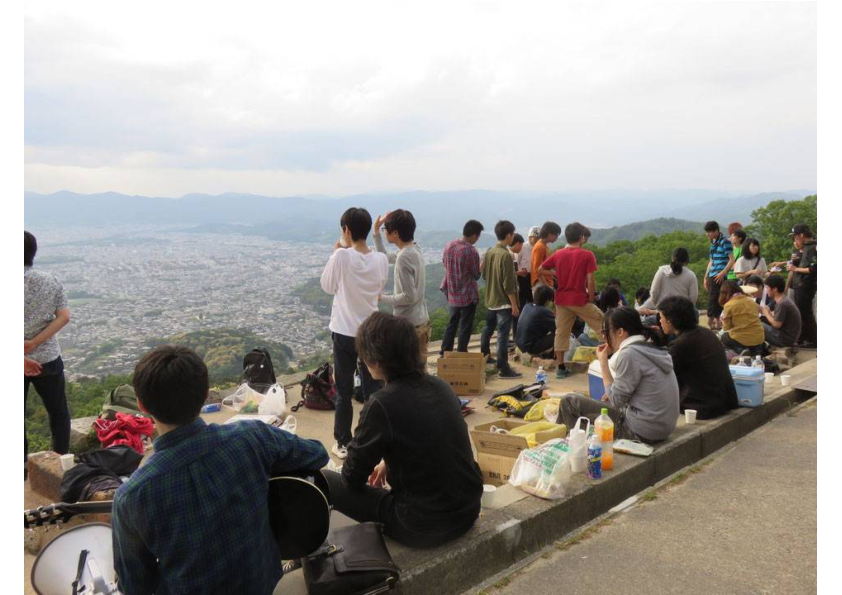
\includegraphics[scale=0.3]{daimonji_1.pdf}
			%\caption{}
			\vspace*{-\intextsep}
			\label{fig:大文字}
			\end{wrapfigure}

 ※どんな企画でも許可されるわけではありませんので, ご了承ください.







\newpage

	\section{くまのまつり ---春の地域祭り}

		\subsection{くまのまつりとは}
		熊野寮では, 毎年5月の下旬に「くまのまつり」というお祭を開催しています. このお祭は, もともとは地域の商店の方々が立ち上げ, 2011年から寮自治会が主催を引き継いだものです. これは地域と一緒につくるお祭りであり, 寮自治会としては寮外との連帯を目指すためのお祭りです.

		お祭りでは地域の飲食店や雑貨店, 個人など20以上の外部出店ブースが並びます. ステージパフォーマンスや子供向けの企画もあり, とにかく楽しいお祭りです. 来場者は2日で1000人ほど. Facebook「\href{https://www.facebook.com/\%e3\%81\%8f\%e3\%81\%be\%e3\%81\%ae\%e3\%81\%be\%e3\%81\%a4\%e3\%82\%8a-789960784504806/}{くまのまつり}」ページにも写真がたくさん載ってます. お祭りの様子は写真を見てもらうのが一番だと思うのでそちらを見てください.

		\subsection{くまのまつりを行う意味}

	\begin{wrapfigure}{r}[0pt]{0.5\textwidth}
		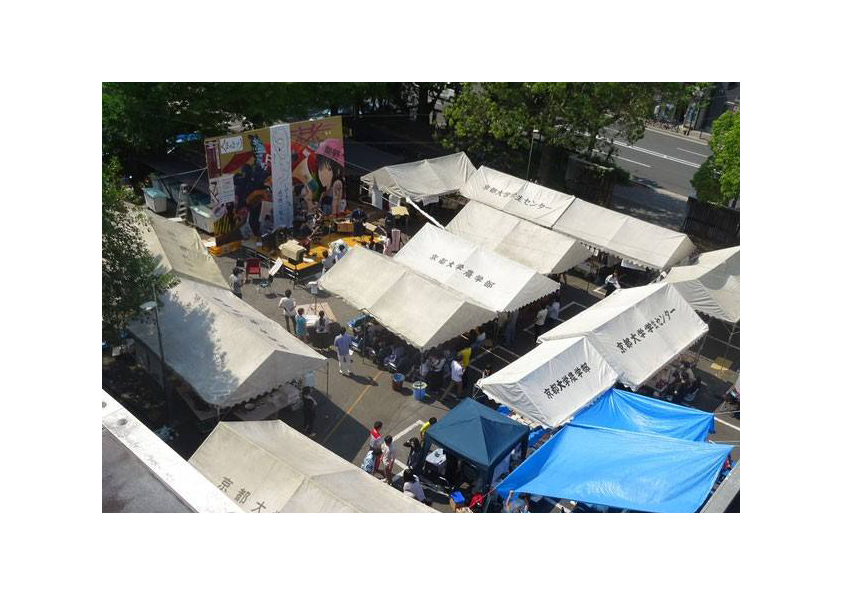
\includegraphics[scale=0.4]{kumano_fes.pdf}
			%\caption{}
			\label{fig:くまのまつり}
			\end{wrapfigure}
		ここでは「くまのまつり」開催の意義を少し掘り下げます. 端的に言えば, 「熊野寮の活動の素晴らしさを外部に発信する場」として「くまのまつり」があります.

		熊野寮では2013年から毎年, 公安警察による熊野寮の家宅捜索が行われています. 2014年からはそれが大々的に全国に報じられるようになり, 寮生も度々逮捕されるようになりました. 家宅捜索の中で公安警察が行う違法行為$ \cdot $ 人権侵害に対して激しく抗議することもあります. 何かとご心配をおかけし, あるいは不安を抱かせているかもしれません. 一部の報道によって「過激派の巣窟」というイメージを持っている方もいるでしょう.

		そもそも私たちは議論によって, 学生による寮の自主管理$ \cdot $ 運営を行っています. これは, ともすれば住人のエゴによる運営に成り下がってしまうものです. しかし, 私たちはエゴではなく, 「京大で学ぶ者に福利厚生を提供する」という熊野寮の役割を果たし, さらにより良い福利厚生のあり方を追求するために議論し, 寮自治会としての行動をとっています. さらに言えば, 教育を受ける権利を保障するための熊野寮は社会的にも必要なものであり, 我々寮自治会の活動は社会的にも必要なものだという自負があるのです.

		例えば, 公安警察に対する激しい抗議には「住んでいる学生の生活と権利を守るため」という意義があります. 安心して暮らせる住居としての熊野寮を守るための行動です. しかし, この行動も「過激派の巣窟」を描く材料にされてしまいます.

 		さて, そこで私たちがお祭りを通してアピールするのは「過激派の巣窟なんかじゃありません」ということなのか. それは違います. 「過激派」という曖昧な言葉によるレッテル貼りに対して全力で否定することに生産性はありません. 寮生が何を考え, 寮自治会がどういう理念をもってその活動を展開しているのか, 見えにくい中身の話を対面で真摯に説明することにこそ意味があります.

 		レッテル貼りの材料にされようとも, 過激に見えるかもしれない抗議を続け, 中核派の学生が住むことも特に問題としない. そういった中には「安心して暮らせる住居を守る」「寮を必要とする学生には住居を保障する」という, 寮自治会が貫くべき理念があります.

 		ともすれば誤解されてしまう, しかし本当は非常に重要な寮自治会の内実を, しっかりと社会に発信し, 地域の方々と顔の見える関係をつくる中で広げていこうというのが「くまのまつり」の取り組みです.

		今でこそ, 盛大なお祭になった「くまのまつり」ですが, はじめからそうだったわけではありません. 寮生や寮外の協力者がお店や知人に呼びかける中で, 毎年少しずつ輪が広がっていき, このような盛大なお祭へと成長していきました. やりたいと思ったことを何でも実行に移せるのが自治寮のいいところです. 「くまのまつり」は自治会のもつ無限の可能性の一つを示す取り組みだと思います. 入寮を検討される皆さんには入寮してもしなくてもぜひ「くまのまつり」に遊びに来てほしいと思います. もっと言えば一緒にお祭をつくりましょう! できれば入寮して一緒にやりましょう!

		皆でアイデアを出し合いながらお祭を創りあげていく過程, ご近所の人と出会い語る中で新たな関係を創りあげていく過程では, かけがえのない団結が生まれます. それが熊野寮をよりよい自治寮に変えていく何よりのエネルギーなのです.
	\begin{figure}[h]
		\begin{flushleft}
 	 	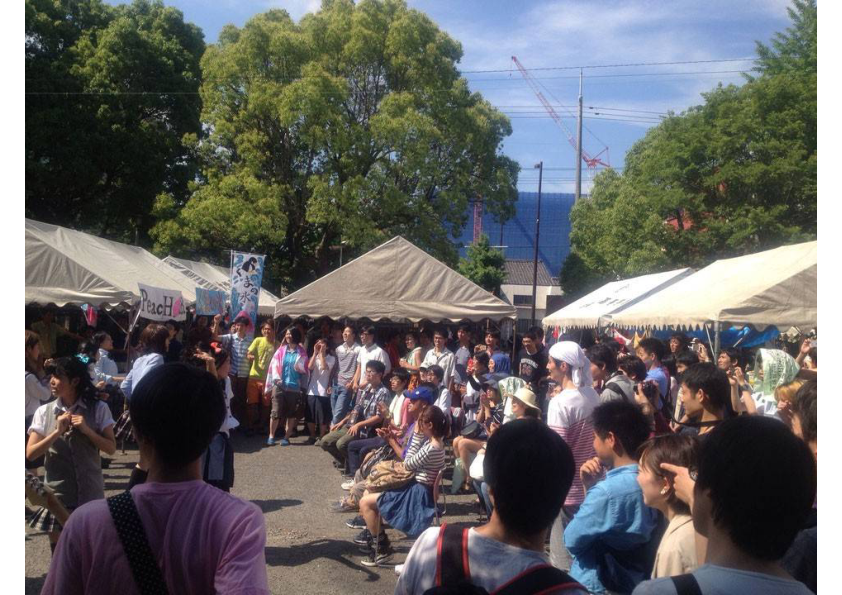
\includegraphics[scale=0.3]{kumano_fes2.pdf}
		\end{flushleft}
		\end{figure}


\newpage

	\section{熊野寮祭 ---厳冬の奇祭}
			\subsubsection{弁明}
			こんにちは. 2018年熊野寮祭実行員長です. この章を読んでいるみなさんにまず弁解なんですが, この文章はコミケ(初参加) の入場待ちの列で寒空のもと, 締め切りに追われて書いたものです. 寒すぎれ指取れそうでした. ゆりかもめ混みスギィ! だから不正確な情報に基づいた記述に基づいたものになるかも知れませんが許して欲しいです. 弁明は以上です.

			\subsubsection{自治と自由とそれからあなた, みんなとがってみんないい}
			まず簡単に熊野寮祭の定番企画を紹介してみなさんの度肝を抜いておきます.
			\begin{description}
			\item[鴨川いかだレース] 12月の鴨川を自作のいかだ(突貫工事で作成) で渡る. いかだが壊れたら泳ぐ.
			\item[四条大運動会] 四条周辺で熊野寮生が運動会をする. 鴨川沿いで綱引したり, 三条から四条まで二人三脚したり. 一般参加も大歓迎. 警察権力からも参加多数.
			\item[大階段グリコ] 京都駅の171段の階段を一般の人とジャンケンしまくってグリコで登る. 羞恥心を捨て去れ.
			\item[AB棟感綱引き]熊野寮のAB棟の間に綱を渡して綱引きをする. AB棟間での煽り合いが見もの.
			\item[時計台コンパ]京大のクスノキ周辺でコンパを開く. 諸事情により2018年は熊野寮D棟(旧称: 時計台) に登らなかった. 次代の時計台占拠はあなたに託された!
			\end{description}

			これ以外にもドッグフードやキャットフードを食べてみたり, 最凶のダサい服でおされな店に出かけてみたり, アルミホイルを何時間も延々と叩き続けたり, 焼畑したり, 薪を割ってお風呂に入ったり, 偽の謝罪会見を開いたりととにかくやりたいことをやってしまうのが熊野寮祭だとわかっていただけるでしょうか.

			熊野寮祭は自由な場です. あなたのやりたいことを止める人はおそらくいないしょう. きっと型どおりではない経験を味わうことになると思います. これは受験生の方に向けて書くのですが, 京都大学というのは存外に普通なところです. 普通に授業を受け, 普通にサボり, 普通にバイトし, 普通にサークルに行く. 京大のいわゆる狂気といえるような人はごく一部にしかいないのです. しかし, ここ熊野寮にはまだ狂気と呼べるものが根強く残っていて, 大学生たちを情熱のままに行動させてしまうのです.

			もしあなたが京都大学というブランドに, 自由と狂気とそれから他の追随を許さない強烈な個性を求めているのなら, 熊野寮祭はその全てを実現することができるでしょう.

			寮祭実行委員長という大仰な役割を仰せつかった私も, 実はまだ一回生です. ですから, 学年なんて関係ありません. あたなの「これをやったらヤバイw」が次代の熊野寮祭を大きく盛り上げて行くことになるでしょう.
あなたの熊野寮祭への参加をこころよりお待ちしております.
\begin{figure}[h]
		\begin{flushleft}
 	 	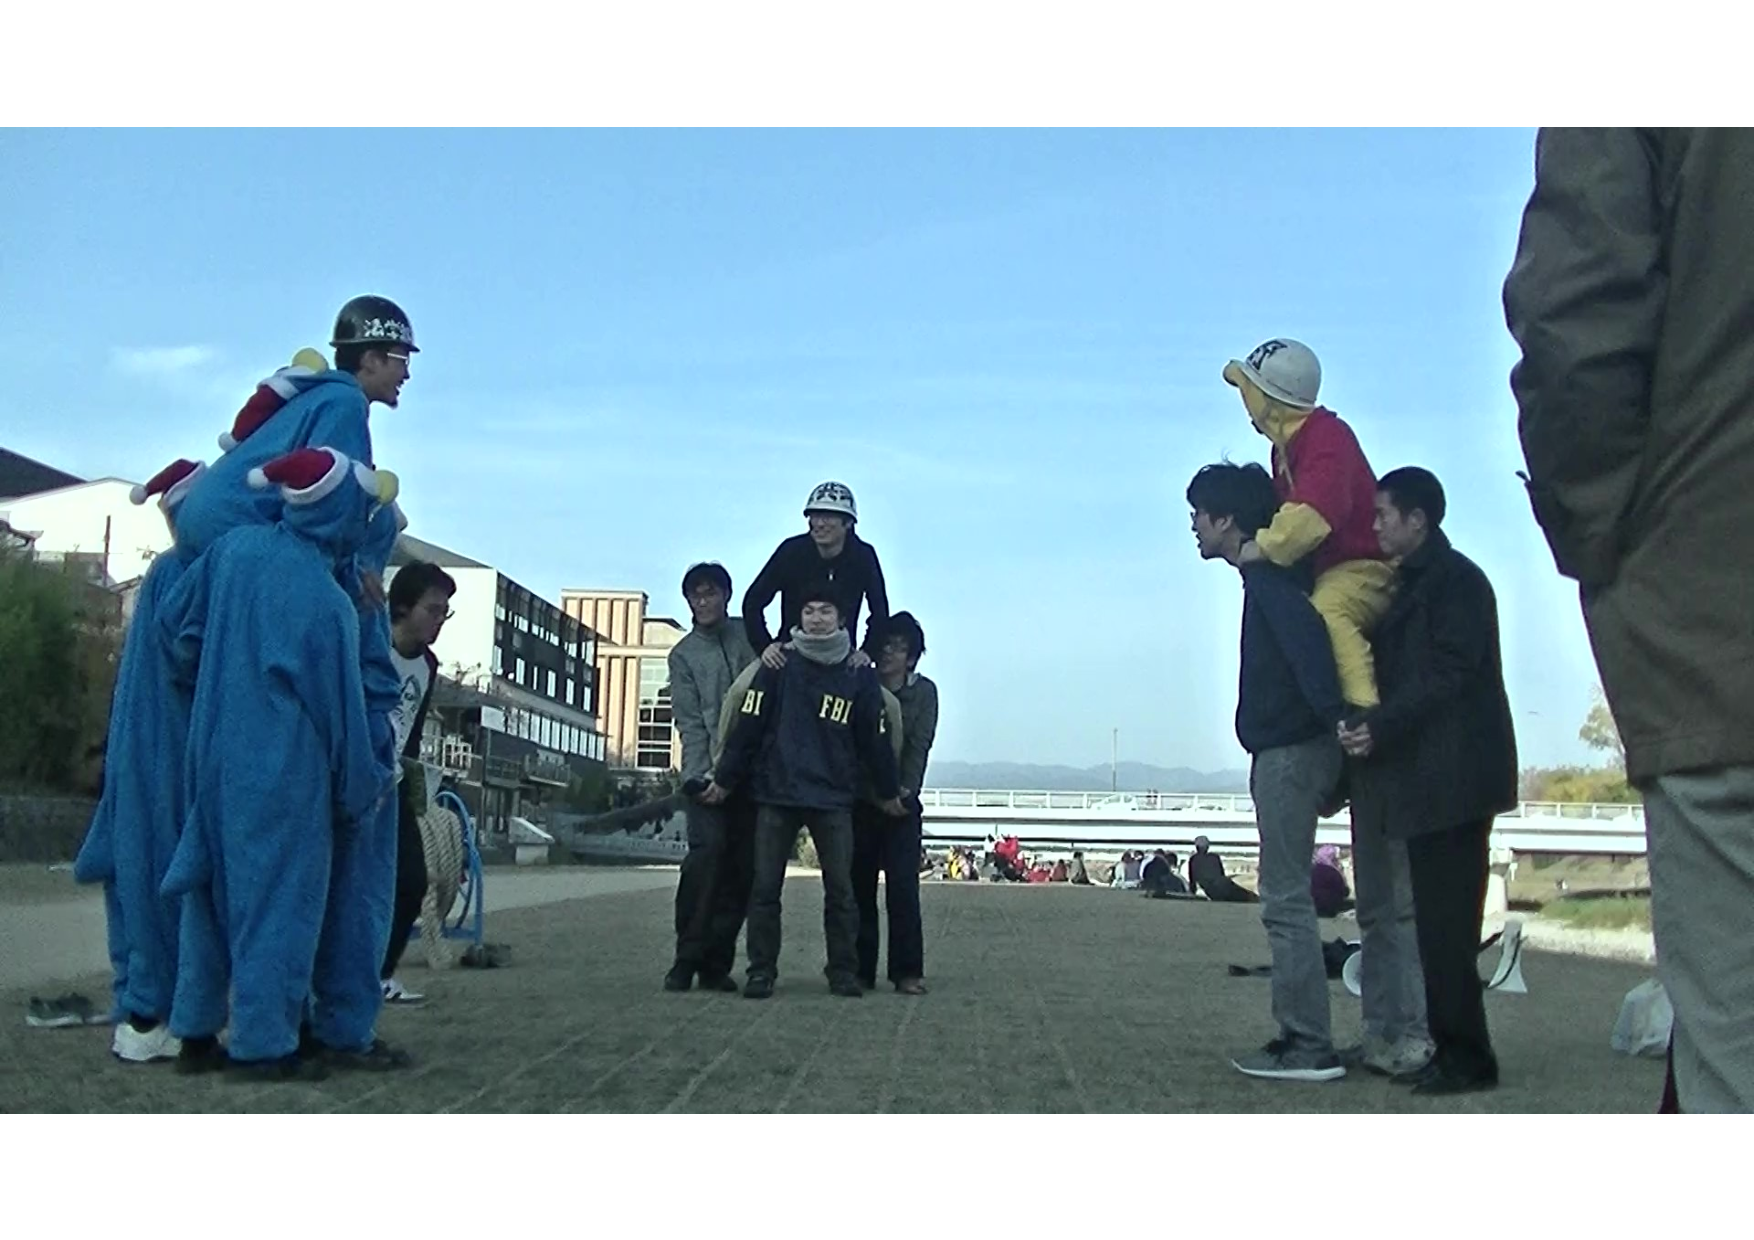
\includegraphics[scale=0.25]{kibasen.pdf}
		\end{flushleft}
		\end{figure}

\end{document}
